This chapter provides a theoretic view of synchronous testing that involve
internal nondeterminsm.  \autoref{sec:concepts} defines the basic concepts in
testing.  \autoref{sec:qac} introduces a language family for writing protocol
specifications and validators.  \autoref{sec:correctness} shows how to reason on
validators' soundness and completeness with respect to the specification.

\section{Concepts}
\label{sec:concepts}
Testers are programs that determine whether implementations are compliant or not
by observing their behavior.  This section defines the basic concepts and
notations in testing.

\begin{definition}[Implementations and Behaviors]
  {\em Implementations} are programs that can interact with their environment.
  {\em Behaviors} are traces of the implementation's interactions with the
  environment and consist of (i) {\em Outputs}, which are performed by the
  implementation and can be observed in the environment, and (ii) {\em Inputs},
  which can be manipulated for testing purposes, causing (potentially) different
  outputs of the implementation.

  ``Implementation $i$ can {\em produce} behavior $b$'' is written as
  ``$\behaves i b$''.
\end{definition}

\begin{definition}[Specifications, Validity, and Compliance]
  A {\em specification} is a description of valid behavior.  ``Behavior $b$ is
  {\em valid} per specification $s$'' is written as ``$\valid s b$''.
  
  An implementation $i$ {\em complies} with a specification $s$ (written
  ``$\complies s i$'') if it only produces behaviors that are valid per the
  specification:
  \[\complies s i\quad\triangleq\quad\forall b,(\behaves i b)\implies\valid s b\]
\end{definition}

\begin{definition}[Tester components and correctness]
  A tester consists of (i) a {\em validator} that accepts or rejects
  implementations' behavior, and (ii) a {\em test harness} that triggers
  different behavior with various input.

  A tester is {\em correct} if its acceptances and rejections are sound and
  complete.  A tester is {\em rejection-sound} if it only rejects incompliant
  implementations; it is {\em rejection-complete} if it can reject all
  incompliant implementations, provided sufficient time of
  execution.\footnote{The semantics of ``soundness'' and ``completeness'' vary
    among contexts.  This paper inherits terminologies from existing
    literature~\cite{Tretmans}, but explicitly use ``rejection-'' prefix for
    clarity.  ``Rejection soundness'' is equivalent to ``acceptance
    completeness'', and vice versa.}

  The tester's correctness is based on its components properties: A
  rejection-sound tester requires its validator to be {\em rejection-sound}; A
  rejection-complete tester consists of (i) a {\em rejection-complete} validator
  and (ii) an {\em exhaustive} test harness that can eventually trigger invalid
  behavior.
\end{definition}

\begin{definition}[Soundness and completeness of validators]
  A validator $v$ is {\em rejection-sound} with respect to specification $s$
  (written as ``$\rejSound v s$'') if it only rejects behaviors that are invalid
  per $s$:
  \[\rejSound v s\quad\triangleq\quad\forall b,\rejects v b\implies\invalid s b\]

  A validator $v$ is {\em rejection-complete} with respect to specification $s$
  (written as ``$\rejComplete v s$'') if it rejects all behaviors that are
  invalid per $s$:
  \[\rejComplete v s\quad\triangleq\quad\forall b,\invalid s b\implies\rejects v b\]
\end{definition}

In property-based testing (PBT)~\cite{pbt}, validators' soundness and
completeness are trivial, because the specification itself defines ``how to
compute whether some behavior is valid or not''.  The validator is identical to
the specification.

Whereas, in model-based testing (MBT)~\cite{broy2005model}, the specification
defines ``how to produce valid behavior''.  The validator needs to compute
whether the observed behavior {\em can be produced} by the specification.

PBT and MBT are different views of the system under test: the former observes
from outside, and the latter abstracts the internal computation.  When the
system might perform nondeterministic behavior, MBT allows specifying the system
in a more reasonable way, which is explained in
\autoref{sec:challenge-nondeterminism}.

\begin{definition}[Exhaustiveness of test harness]
  A test harness $h$ is {\em exhaustive} with respect to specification $s$
  (written as ``$\exhaustive s h$'') if, for any implementation that does not
  comply with the specification, the test harness can eventually trigger some
  invalid behavior to reveal such incompliance:
  \begin{align*}
    \exhaustive s h\quad\triangleq\quad\forall i,\;&\ncomplies s i \\
    &\implies \exists b,(\triggers i h b)\wedge\invalid s b
  \end{align*}
\end{definition}

Exhaustive test harnesses can be built na\"ively by enumerating all test cases.
However, to capture bugs within realistic budget, the test harness should
produce test cases that are (i) more likely to trigger bugs, and (ii) of minimal
size to help analyzing and locating the bug.  These challenges are further
discussed in \autoref{sec:challenge-harness}.


\section{QAC language family}
\label{sec:qac}
In this section, I introduce the ``query-answer-choice'' (QAC) language family
for writing specifications and validators for network protocols that involve
internal nondeterminism.

\subsection{Specifying protocols with server models}
\label{sec:qac-model}
Network protocols can be specified with ``reference implementations'' {\it i.e.}
model programs that exhibit the space of valid behaviors.  For client-server
systems such as WWW, we can specify networked servers as programs that receive
queries and compute the responses.  Here I model the server programs with a data
structure called state monad.

\begin{definition}[State monad]
  Let $S$ be the state type, $A$ be the result type, then type $(S\to A\times
  S)$ represents a computation that, given a pre state, yields a result and the
  post state.  This computation is pronounced a ``state monad with state type
  $S$ and result type $A$''.

  For example, let the state be a key-value mapping $(K\to V)$, then we can
  define \ilc{get} and \ilc{put} computations as follows:
  \begin{align}
    \tag{1}&\mathtt{get}:K\to((K\to V)\to V\times(K\to V))\\
    \tag{2}&\mathtt{get}(k)(f)\triangleq (f(k), f)\\
    \tag{3}&\mathtt{put}:K\times V\to((K\to V)\to ()\times(K\to V))\\
    \tag{4}&\mathtt{put}(k,v)(f)\triangleq((),\update f k v)
  \end{align}

  These function definitions should be read as:
  \begin{enumerate}
    \item The \ilc{get} function takes a key as argument, and constructs a
      state monad with state type $(K\to V)$ and result type $V$.
    \item Given argument $k$ of type $K$, $\mathtt{get}(k)$ takes a mapping $f$
      as pre state and yields the mapped value $f(k)$ as result.  The post state
      is the original mapping $f$ unchanged.
    \item The \ilc{put} function takes a key-value pair as argument, and
      constructs a state monad with state type $(K\to V)$ and result type
      ``$()$'' (unit type, which corresponds to \inlinec{void} return type in
      C/Java functions).
    \item Given argument $(k,v)$ of type $(K\times V)$, $\mathtt{put}(k,v)$
      takes a mapping $f$ as pre state and substitues its value at key $k$ with
      $v$.  The post state is the substituted mapping $\update f k v$.
  \end{enumerate}
\end{definition}

Now we can define the server model in terms of state monad:

\begin{definition}[Deterministic server model]
  \label{def:qaserver}
  A deterministic server is an infinite loop whose loop body takes a query and
  produces a response.  The server definition consists of the loop body and a
  current state:
  \[\mathsf{DeterministicServer}\triangleq\sigT{S}{(Q \to S \to A \times S) \times S}\]
  This type definition is pronounced as: A deterministic server has an initial
  state of some type $S$.  Its loop body takes a request of type $Q$ and
  computes a state monad with state type $S$ and result type $A$, where type $A$
  represents the response.

  Notice that the server's state type is existentially quantified~\cite{tapl},
  while its query and response types are not.  This is because a protocol
  specification only defines the space of valid traces, and doesn't require the
  implementation's internal state to be a specific type.

  An instance of server model is written as:
  \[\existT S \sigma (\sstep,state_0)\]
  This expression is pronounced as: The server state is of type $\sigma$.  Its
  loop body is function $\sstep$ (which has type $Q\to\sigma\to A\times\sigma$)
  and its initial state is $state_0$ (which has type $\sigma$).
\end{definition}

For example, consider a compare-and-set (CMP-SET) protocol: The server stores a
number \inlinec n.  If the client sends a request that is smaller than \inlinec
S, then the server responds with \inlinec 0.  Otherwise, the server sets
\inlinec n to the request and responds with \inlinec 1:
\begin{lstlisting}[style=customc]
  int n = 0;
  while (true) {
    int request = recv();
    if (request <= n) send(0);
    else { n = request; send(1); }
  }
\end{lstlisting}

Such a server can be modelled as:
\begin{align*}
  \existT{S}{\Int}{(&\lam{(q)(n)}{\begin{cases}
        (0,s)&q\le n\\
        (1,q)&\mathrm{otherwise}
    \end{cases}},\\
    &0)}
\end{align*}

In general, servers' responses and transitions might depend on choices that are
invisible to the testers, so called internal nondeterminism, as discussed in
\autoref{sec:internal-nondeterminism}.  I represent the space of nondeterminstic
behaviors by parameterizing it over the server's internal choice.

\begin{definition}[Nondeterministic server model]
  \label{def:server}
  A nondeterministic server is an infinite loop whose loop body takes a query
  and an internal choice to produce a responses.  The nondeterministic server
  definition extends \autoref{def:qaserver} with a choice argument of type $C$:
  \[\Server\triangleq\sigT S{(Q\times C\to S\to A\times S)\times S}\]
\end{definition}

Consider changing the aforementioned CMP-SET into compare-and-reset (CMP-RST):
When the request is greater than \inlinec S, the server may reset \inlinec S to
any arbitrary number:
\begin{lstlisting}[style=customc]
  int arbitrary();
  int n = 0;
  while (true) {
    int request = recv();
    if (request <= n) send(0);
    else { n = arbitrary(); send(1); }
  }
\end{lstlisting}
Its corresponding server model can be written as:
\begin{align*}
  \existT{S}{\Int}{(&\lam{(q,c)(n)}{
      \begin{cases}
        (0,n)& q\le n\\
        (1,c)&\mathrm{otherwise}
      \end{cases}
    },\\
    &0)}
\end{align*}
This model represents the space of uncertain behavior with the internal choice
parameter of type integer.  For any value $(c:\Int)$, the server is allowed to
reset $S$ to $c$.

\subsection{Valid traces of a server model}
By specifying protocols with server models, we can now instantiate the trace
validity notation ``$\valid s t$'' in \autoref{def:compliance} in terms of
operational semantics.

\begin{definition}[Server transitions]
  \label{def:server-step}
  Upon request $q$ and choice $c$, server model $s$ can step to $s'$ yielding
  response $a$ (written ``$\triggers sc{(q,a)}s'$~'') if and only if the
  response and the post model can be computed by the $\stepServer$ function:

\begin{align*}
  &\triggers sc{(q,a)}s'\quad\triangleq\quad\stepServer(q,c)(s)=(a,s')\\
  &\stepServer:Q\times C \to \Server \to A\times \Server \\
  &\stepServer(q,c)(s)\triangleq\\
  &\qquad\letin{(\existT{S}{\sigma}{(\sstep, state)})}{s}\\
  &\qquad\letin{(a,state')}{\sstep(q,c)(state)} \\
  &\qquad(a, \existT{S}{\sigma}{(\sstep, state')})
\end{align*}

The $\stepServer$ function takes a query and a choice and computes a state monad
with state type $\Server$ and result type $A$, by pattern matching on argument
$(s:\Server)$.  Let $\sigma$ be the server state type of $s$, $\sstep$ be the
loop body, and $(state:\sigma)$ be the current state of $s$, then
$\stepServer(q,c)(s)$ computes the result $(a:A)$ and the post state
$(state':\sigma)$ using the $\sstep$ function, and substitutes the server's
pre-step $state$ with the post-step $state'$.
\end{definition}

\begin{definition}[Trace validity in QAC]
  \label{def:trace-validity}
  In the QAC language family, a trace is a sequence of $Q\times A$ pairs.  When
  specifying a protocol with a $\Server$ model, a trace $t$ is valid per
  specification $s$ if and only if it can be {\em produced} by the server model:
  \[\valid s t\quad\triangleq\quad\exists s',\behaves s t s'\]
  Here the producibility relation in \autoref{sec:concepts} is expanded with an
  argument $s'$ representing the post-transition state, pronounced
  ``specification $s$ can produce trace $t$ and step to specification $s'$~'':
  \begin{enumerate}
  \item A server model can produce an empty trace and step to itself:
    \[\behaves s \nil s\]
  \item A server model can produce a non-empty trace if it can produce the head
    of the trace, and step to some server model that produces the tail of the
    trace:
    \[\behaves s {t+(q,a)} s_2\quad\triangleq\quad\exists s_1,c,\behaves s t s_1\wedge\triggers {s_1}c{(q,a)}s_2\]
  \end{enumerate}
\end{definition}

\subsection{Validating traces}
The validator takes a trace and determines whether it is valid per the protocol
specification.

\begin{definition}[Validator]
A validator is an infinite loop whose loop body takes a pair of query and
response and determines whether it is valid or not.  The validator iterates over
a state of some type $V$.  Given a $Q\times A$ pair, the loop body may return a
next validator state or return nothing, written as type ``$\option V$'':
\[\begin{array}{lll}
  \Validator&\triangleq&\sigT{V}{(Q\times A\to V\to\option V)\times V}\\
  \option X&\triangleq&\Some(x:X)\mid\None
\end{array}\]
\end{definition}

For example, a validator for the CMP-SET protocol is written as:
\begin{align*}
  \existT{V}{\Int}{(&\lam{(q,a)(v)}{
      \begin{cases}
        \If a\Is 1\Then\Some v\Else\None&q\le v\\
        \If a\Is 1\Then\Some q\Else\None&\mathrm{otherwise}
      \end{cases}
    },\\
    &0)}
\end{align*}
Here the validator state the same as the server model's.  The loop body computes
the expected response and compares it with the observed response.  If they are
the same, then the next server state is used as the next validator state.
Otherwise, the function returns $\None$, indicating that the response is
invalid.

Having defined the validator type, we can now instantiate the trace acception
notation ``$\accepts v t$'' in \autoref{def:tester} in terms of operational
semantics.

\begin{definition}[Validator transitions]
  \label{def:validator-step}
  Validator $v$ can consume request $q$ and response $a$ and step to $v'$
  (written ``$\behaves v{(q,a)}v'$~'') if and only if the post validator can be
  computed by the $\stepValidator$ function:
\begin{align*}
  &\behaves v{(q,a)}v'\quad\triangleq\quad\stepValidator(q,a)(v)=\Some v'\\
  &\stepValidator:Q\times A\to\Validator\to\option\Validator\\
  &\stepValidator(q,a)(\existT{V}{\beta}{(\vstep,state)})\\
  &\qquad\triangleq\begin{cases}
  \Some{(\existT{V}{\beta}{(\vstep,state')})} & \vstep(q,a,state)=\Some{state'} \\
  \None & \vstep(q,a,state)=\None
  \end{cases}
\end{align*}
The $\stepValidator$ function takes a query and a response, and computes the
validator transition by pattern matching on argument $(v:\Validator)$.  Let
$\beta$ be the validator state type of $v$, $\vstep$ be the loop body, and
$(state:\beta)$ be the current state of $v$, then $\stepValidator(q,a)(v)$ calls
the $\vstep$ function to validate the $Q\times A$ pair.  If the pair is valid,
then $\vstep$ returns a post-validation $state'$, which replaces the validator's
current $state$.  Otherwise, the validator halts with $\None$.
\end{definition}

\begin{definition}[Trace acceptance in QAC]
A validator accepts a trace if it cosumes the entire trace:
\[\accepts v t\quad\triangleq\quad\exists v',\behaves v t v'\]
\begin{enumerate}
\item A validator can consume an empty trace and step to itself:
  \[\behaves v\nil v\]
\item A validator consumes a non-empty trace if it can consume the head of the
  trace, and step to some validator that consumes the tail of the trace:
  \[\behaves v {t+(q,a)} v_2\quad\triangleq\quad\exists v_1,\behaves v t v_1\wedge
  \behaves{v_1}{(q,a)}{v_2}\]
\end{enumerate}
\end{definition}


\section{Soundness and completeness of validators}
\label{sec:correctness}
We can now phrase the correctness properties in \autoref{sec:concepts} in terms
of the QAC language family:
\begin{enumerate}
  \item A rejection-sound ({\it i.e.} acceptance-complete) validator consumes
    all traces that are producible by the protocol specification:
    \[\begin{array}{lrl}
      \rejSound v s&\triangleq&\forall t,\rejects v t\implies\invalid s t\\
      &\triangleq&\forall t,(\exists s',\behaves s t s')\implies\exists v',\behaves v t v'
    \end{array}\]
  \item A rejection-complete ({\it i.e.} acceptance-sound) validator only
    consumes traces that are producible by the protocol specification:
    \[\begin{array}{lrl}
      \rejComplete v s&\triangleq&\forall t,\invalid s t\implies\rejects v t\\
      &\triangleq&\forall t,(\exists v',\behaves v t v')\implies\exists s',\behaves s t s'
    \end{array}\]
\end{enumerate}

Both the specification and the validator are infinite loops.  To show that the
validator consumes the same space of traces as the specification produces, we
need to show the correspondence between each server and validator step.  This is
done by introducing some loop invariant between the server and validator states,
and show that it is preserved by the server's and the validator's loop body.

\subsection{Proving rejection soundness}
To prove that any trace producible by server $\existT{S}{\sigma}{(\sstep,s_0)}$
is consumable by validator $\existT{V}{\beta}{(\vstep,v_0)}$, I perform forward
induction on the server's execution path, and show that every step has a
corresponding validator step:
\begin{itemize}
\item The initial server state $s_0$ simulates the initial validator state $v_0$:
  \begin{equation}
    \tag{RejSound-Init}
    \label{eq:rs1}
    \Reflects{(v_0:\beta)}{(s_0:\sigma)}
  \end{equation}
\item Any server step $\sstep(q,c,s)=(a,s')$ whose pre-execution state $s$
  reflects some pre-validation state $v$ can be consumed by the validator
  yielding a post-validation state $v'$ that reflects the post-execution state $s'$:
  \begin{align*}
    \tag{RejSound-Step}
    \label{eq:rs2}
    &\forall(q:Q)(c:C)(a:A)(s,s':\sigma)(v:\beta),\\
    &\sstep(q,c,s)=(a,s')\wedge\Reflects{v}{s}\\
    &\implies\exists v':\beta,\vstep(q,a,v)=\Some{v'}\wedge\Reflects{v'}{s'}
  \end{align*}
  \begin{center}
    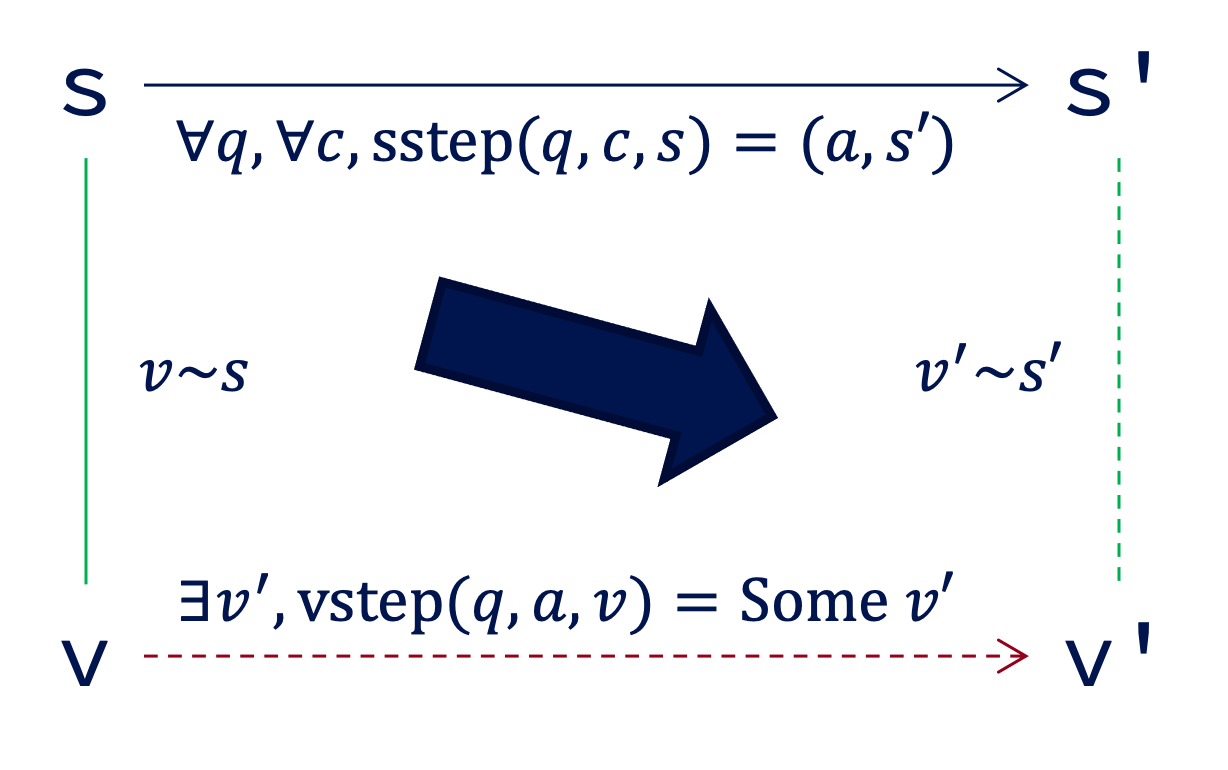
\includegraphics[width=.5\textwidth]{figures/sound}
  \end{center}
\end{itemize}

\subsection{Proving rejection completeness}
To prove that any trace consumable by validator
$\existT{V}{\beta}{(\vstep,v_0)}$ is producible by server
$\existT{S}{\sigma}{(\sstep,s_0)}$, we need backward induction on the
validator's execution path and show that every step has a corresponding server
step:
\begin{itemize}
\item Any accepting validator step $\vstep(q,a,v)=\Some v'$ has some server
  state $s'$ that reflects the post-validation state $v'$:
  \begin{align*}
    \tag{RejComplete-End}
    \label{eq:rc1}
    \forall(q:Q)(a:A)(v, v':\beta),\;&\vstep(q,a,v)=\Some{v'}\\
    &\implies\exists s':\sigma,\Reflects{v'}{s'} 
  \end{align*}
\item Any accepting validator step $\vstep(q,a,v)=\Some v'$ whose
  post-validation state $v'$ reflects some post-execution server state $s'$
  has a corresponding server step from a pre-execution state $s$
  that reflects the pre-validation state $v$:
  \begin{align*}
    \tag{RejComplete-Step}
    \label{eq:rc2}
    &\forall(q:Q)(a:A)(v,v':\beta)(s':\sigma),\\
    &\vstep(q,a,v)=\Some{v'}\wedge\Reflects{v'}{s'}\\
    &\implies\exists(s:\sigma)(c:C),\sstep(q,c,s)=(a,s')\wedge\Reflects{v}{s}
  \end{align*}
  \begin{center}
    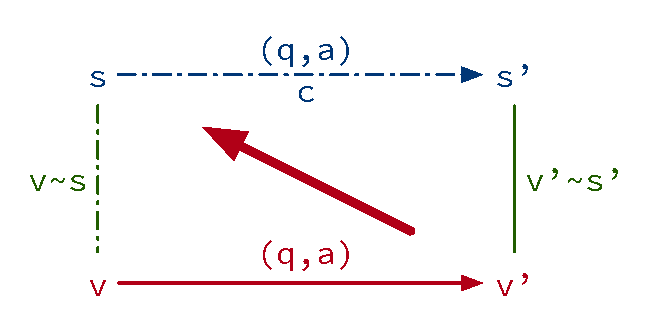
\includegraphics[width=.5\textwidth]{figures/complete}
  \end{center}

\item The initial validator state $v_0$ only reflects the initial server state $s_0$:
  \begin{equation}
    \tag{RejComplete-Init}
    \label{eq:rc3}
    \{s\mid\Reflects{v_0}{s}\}=\{s_0\}
  \end{equation}
\end{itemize}

Rejection soundness is proven by forward induction, while rejection completeness
is proven by backward induction.  This is because the choice $C$ is known from
the server step, but unknown from the validator step: Given a validator step, we
cannot predict ``what choices the server will make in the future'', but can
analyze ``what choices the server might have made in the past''.  This proof
strategy is further explained with the $\Prog$ example.

